\graphicspath{{anexos/AnexoC-Flame-Diagram/recursos/}}

\section{Comparativa del rendimiento del sistema. Visión general} \label{Anexo:flame-diagram}

En la \autoref{sec:4:mejorando-eficiencia} se plantean diferentes gráficas para analizar y comparar el rendimiento del sistema \legacy{} frente al sistema construido para este TFM. Sin embargo, debido a limitaciones de tamaño de página, no se ha podido incluir lo que es el formato más empleado en este tipo de comparativas, el llamado \textit{Flame Diagram} (llamado así por su forma similar a una llamarada). Esta gráfica resume el \textit{Method Profiling}, explicado en la sección referenciada previamente, de una forma más visual, donde podemos observar además del número de llamadas, cada uno de los métodos de forma jerarquizada, según ciertos métodos invoquen a otros.

Gracias a esto, podemos analizar el porcentaje de cómputo que el sistema emplea para cada método o parte del sistema, pudiendo identificar de una forma sencilla los llamados \textit{hot code-paths}, ``caminos'' del código que más veces se ejecutan y por consiguiente más cómputo requieren.

A continuación se incluye los dos diagramas de llama para sendos sistemas. Se destacan los porcentajes relativos al cómputo del fitness y de la búsqueda. Para el sistema \legacy{} el cómputo de restricciones es del 94.91\% mientras que en el sistema construido es del 25.10\%.

En el diagrama podemos observar dos partes, cada una representa un hilo de ejecución específico, el del sistema en general y el creado en cada llamada a la función de evaluación (fitness) para la paralelización del cómputo del subobjetivo \ref{O2}: el conteo del número de restricciones incumplidas (las incluidas en la \autoref{sec:4:RD}). Además del propio cómputo paralelizado, también se requiere de una cierta cantidad de procesamiento para aunar estos hilos y agrupar el número de restricciones, así como computar el resto del fitness. Esta es la razón por la que aparece en dos lugares en el diagrama, marcados en negro y en morado.
Por último, en verde se han indicado la localización del hilo de ejecución del sistema en sí, \sa{} para el sistema \legacy{}, \vns{} para el sistema final.

\begin{landscape}
	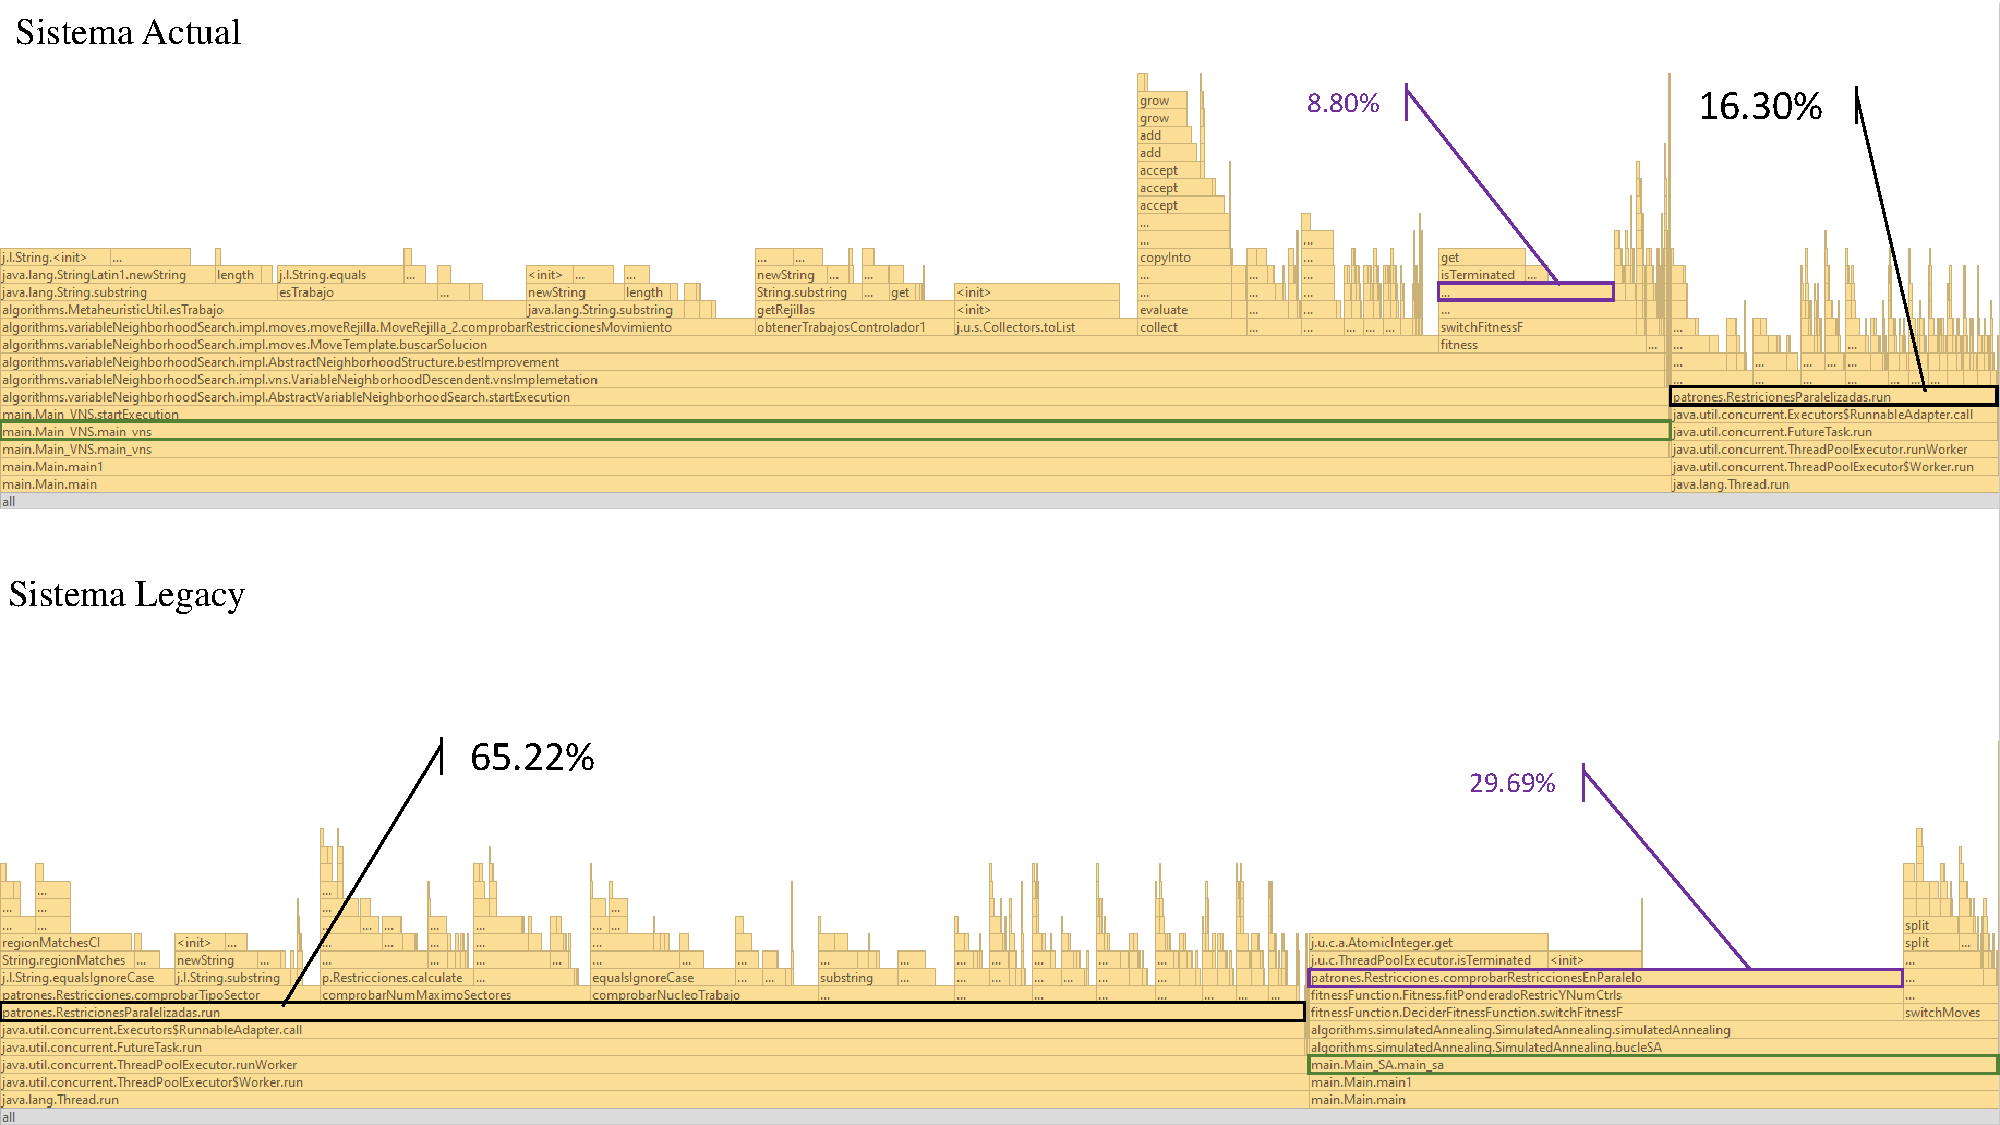
\includepdf[landscape=True]{Flame-diagram}
\end{landscape}
